\documentclass[12pt]{article}

\usepackage{pstricks}
\usepackage{pst-pdf}
\usepackage{pstricks-add}

\pagestyle{empty}

\begin{document}

\psset{unit=1cm,arrowscale=2,linewidth=3pt,linecolor=blue,nodesep=3pt}
\begin{pspicture}(-7,-4)(7,4)%
  %Define locations for all the pins
  \cnode[linewidth=0,linecolor=white](0,0){0.4}{A}
  \cnode[linewidth=0,linecolor=white](1.8,.2){0.4}{B}
  \cnode[linewidth=0,linecolor=white](0.7,1.05){0.4}{C}
  \cnode[linewidth=0,linecolor=white](-.2,1.8){0.4}{D}
  \cnode[linewidth=0,linecolor=white](-1.4,1.2){0.4}{E}
  \cnode[linewidth=0,linecolor=white](-1.8,-.1){0.4}{F}
  \cnode[linewidth=0,linecolor=white](-1.1,-1.5){0.4}{G}
  \cnode[linewidth=0,linecolor=white](0.2,-1.8){0.4}{H}
  \cnode[linewidth=0,linecolor=white](0.8,-0.8){0.4}{J}
 
  %Overlay the graphic of the 9-pin connector
  \rput(0,0){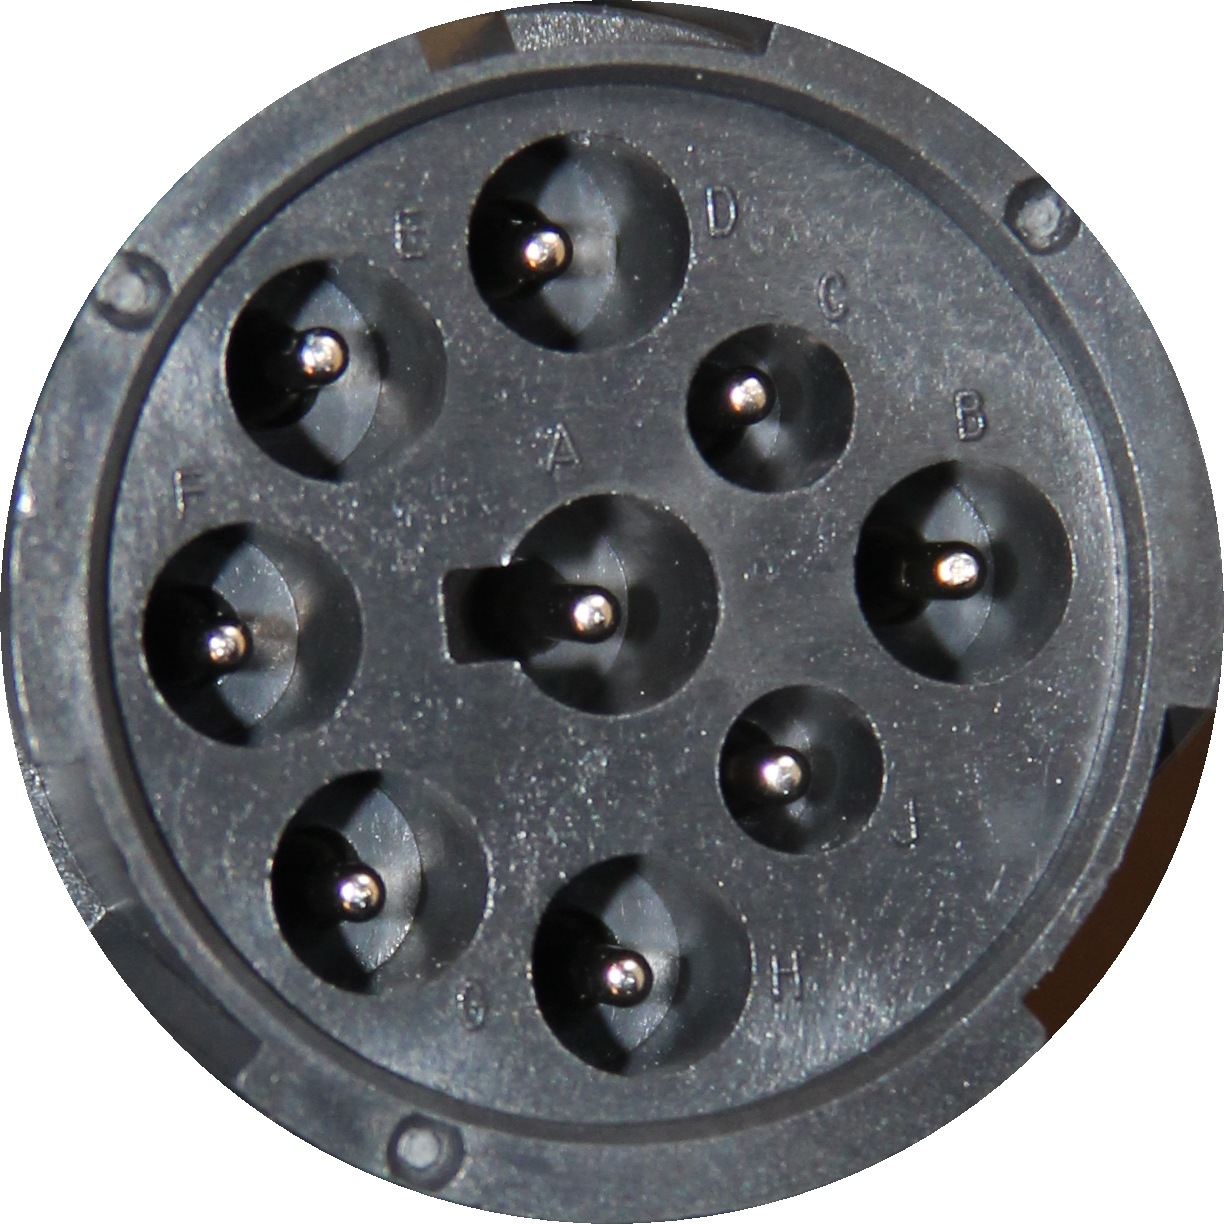
\includegraphics[width=6cm]{9-pin_close_up}}

  %Use the grid to help with alignment of labels and nodes.
  %\psgrid[gridcolor=lightgray]
  
  \uput{4cm}[40](0,0){\rnode{GND}{\Large{A: Ground}}}
  \uput{4cm}[0](0,0){\rnode{+12}{\Large{B: +12V DC}}}
  \uput{4cm}[20](0,0){\rnode{CAN1H}{\Large{C: J1939 High}}}
  \uput{4cm}[140](0,0){\rnode{CAN1L}{\Large{D: J1939 Low}}}
  \uput{4cm}[166.7](0,0){\rnode{CANshld}{\Large{E: J1939 Shield}}}
  \uput{4cm}[193.4](0,0){\rnode{J1708+}{\Large{F: J1708 P}}}
  \uput{4cm}[220](0,0){\rnode{J1708-}{\Large{G: J1708 N}}}
  \uput{4cm}[-40](0,0){\rnode{CAN2H}{\Large{H: CAN2 High}}}
  \uput{4cm}[-20](0,0){\rnode{CAN2L}{\Large{J: CAN2 Low}}}
 
 
  %place curves and connectors to show the different labels
  \nccurve[angleA=80,angleB=180]{<-}{A}{GND}
  \nccurve[angleA=0,angleB=180]{<-}{B}{+12}
  \nccurve[angleA=20,angleB=180]{<-}{C}{CAN1H}
  \nccurve[angleA=140,angleB=0]{<-}{D}{CAN1L}
  \nccurve[angleA=180,angleB=0]{<-}{E}{CANshld}
  \nccurve[angleA=200,angleB=0]{<-}{F}{J1708+}
  \nccurve[angleA=220,angleB=0]{<-}{G}{J1708-}
  \nccurve[angleA=-40,angleB=180]{<-}{H}{CAN2H}
  \nccurve[angleA=-20,angleB=180]{<-}{J}{CAN2L}
  
\end{pspicture}

% can be foo.jpg or .png

\end{document}